\chapter{Testing}\label{ch:testing}

\section{Setup}
All the components listed in Section \ref{ch:compSpec} were mounted on the PCB (can be seen on Fig. \ref{fig:SETUP}) and all the driver circuit were built to be connected to the full setup.
Standard lab power supplies were used to deliver all the inputs needed to the op-amps, SKYPER boards and the input voltage of the circuit itself. 
The maximum output current of the power supply is 3.2A.
For the load a rheostat was used, so that the load can be adjusted to the capabilities of the power supply and the resistance it was set to for the tests was 2.5k$\Omega$ . 

\begin{figure}[H]
	\begin{center}
   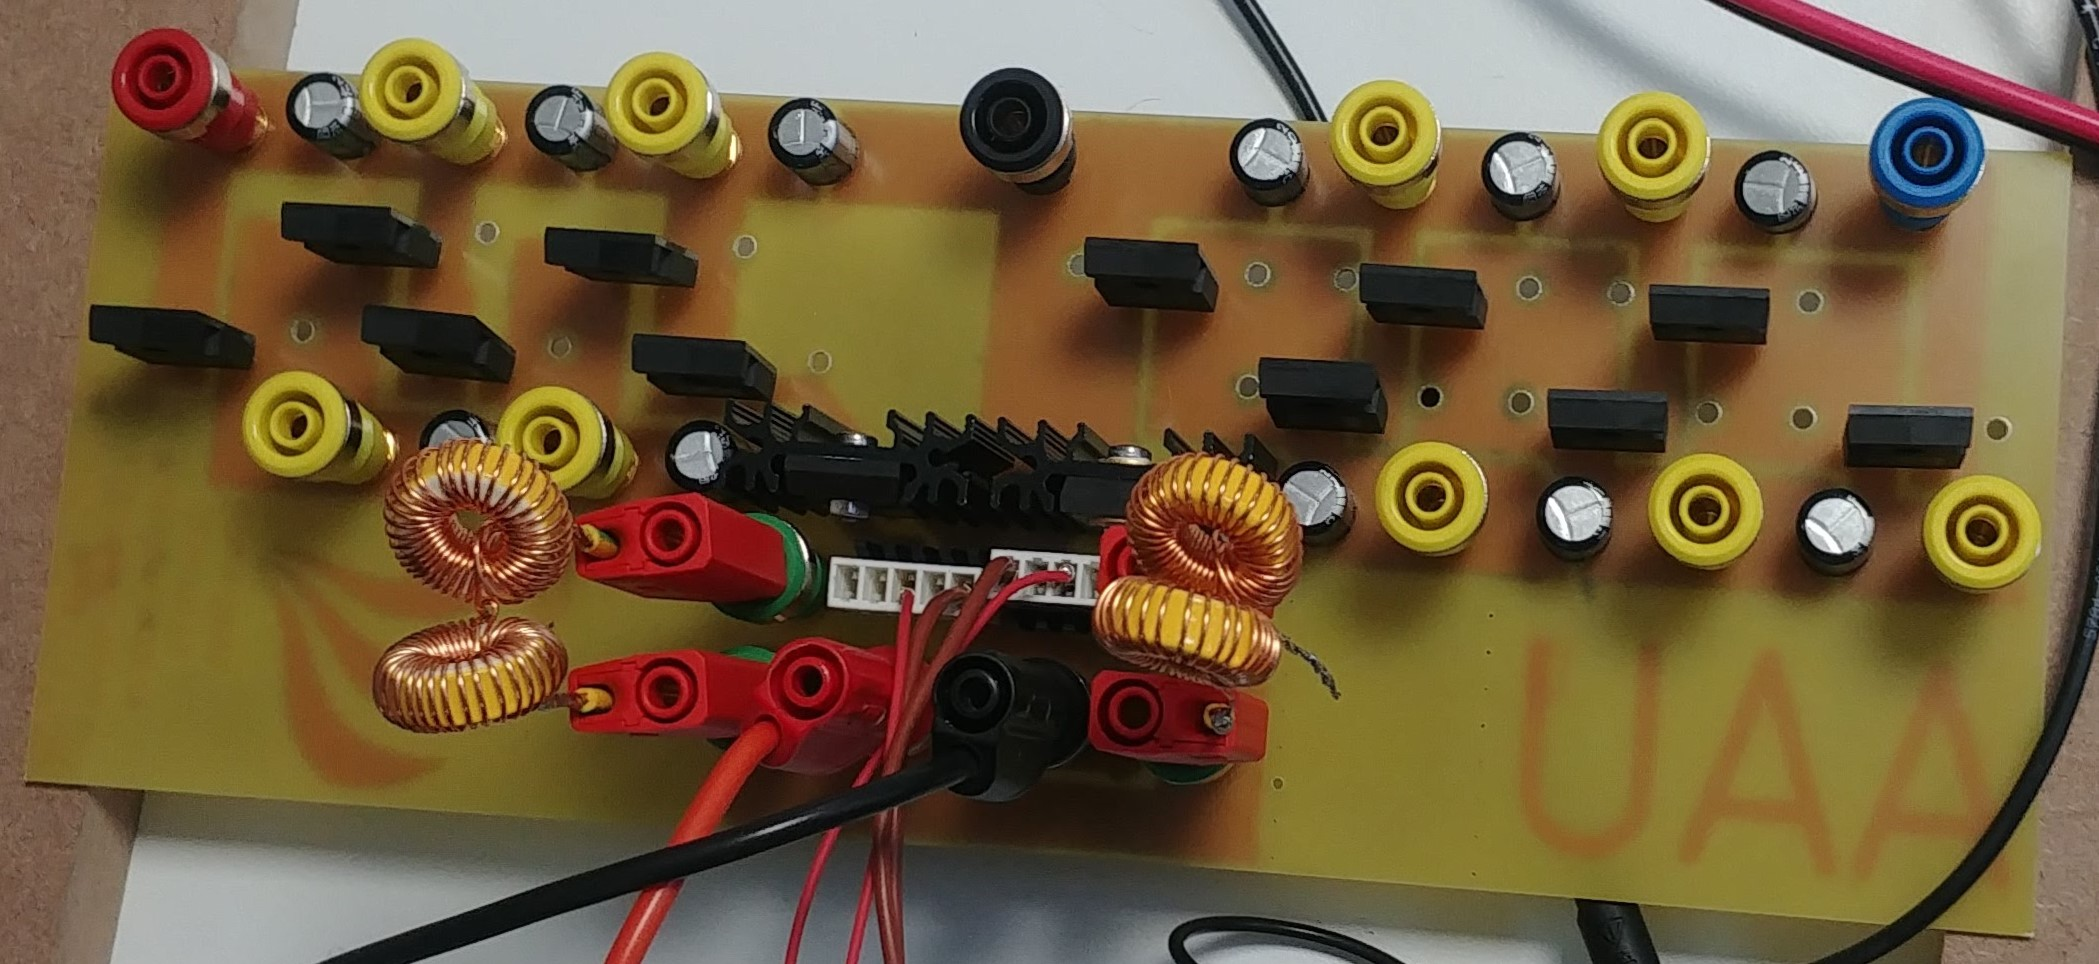
\includegraphics[width=0.8\textwidth]{figures/06Testing/setup.jpg}
	\end{center}
	\vspace{-4mm}
	\caption{PCB with all the components mounted}
	\label{fig:SETUP}
\end{figure}

To generate the PWM input, two wave generators were used, due to the easy synchronisation. The tools used for measurements were ... Oscilloscopes and ... multimeters, all available for us in the AAU Esbjerg laboratories. All the data presented in the next section has been captured in this devices, results comply with their accuracy.
\todo {names of scopes} 
\clearpage
\vspace{-6mm}
\section{Results}

After the setup was complete the first test ran, to test the overall output voltage of the topology within the range of possible duty cycles. The purpose of this tests is too see if the expected gain is matched and what part of the differences are expected and what the unexpected ones can be justified by. 
\vspace{-4mm}

\begin{figure}[H]
	\begin{center}
   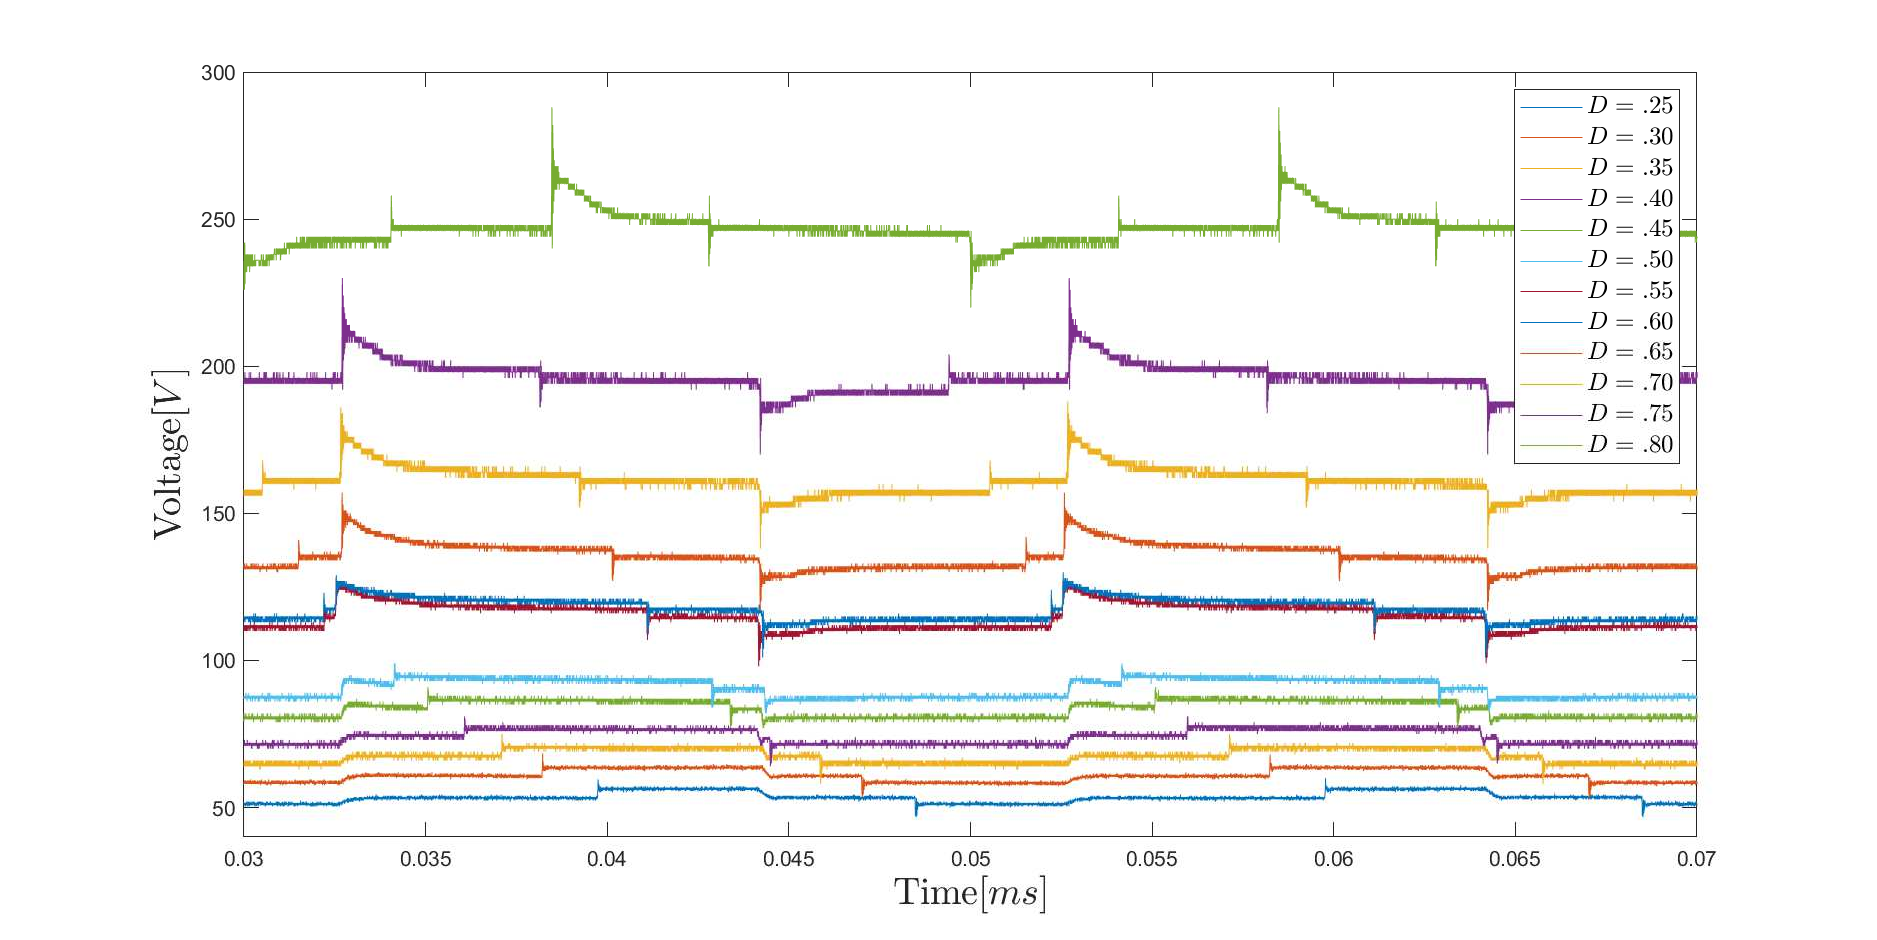
\includegraphics[width=\textwidth]{figures/06Testing/Vripple10Vin.pdf}
	\end{center}
	\vspace{-8mm}
	\caption{$V_o$ at duty cycles between 0.25 and 0.8}
	\label{fig:V_OUT_ALL}
\end{figure}
\vspace{-4mm}
All the output voltage waves can be seen on Fig. \ref{fig:V_OUT_ALL}. To put those values, they need to be compared to the expected values from the expressions we've already derived. All of the calculated and measured values can be seen in the Table \ref{tab:V_OUT_ALL}.
\vspace{-2mm}

\begin{table}[H]
\begin{center}
\caption {Calculated and Measured output voltages} \label{tab:V_OUT_ALL} 
\vspace{-1mm}
\begin{tabular}{|l|l|l|l|}
\cline{1-4}
Duty cycle & Calculated $V_o$ & Measured $V_o$& Difference \\ \cline{1-4}
0.25&	63.92V & 52.59V & 11.31V \\ \cline{1-4}
0.30&	70.00V & 59.7V & 10.30V \\ \cline{1-4}
0.35&	75.936V & 66.1V & 9.836V \\ \cline{1-4}
0.40&	82.86V & 71.8V & 11.06V \\ \cline{1-4}
0.45&	92.15V & 76.40V & 15.746V \\ \cline{1-4}
0.50&	102.4V & 83.3V & 19.10V \\ \cline{1-4}
0.55&	114.934V & 93.1V & 21.834V \\ \cline{1-4}
0.60&	125V & 106.80V & 18.20V\\ \cline{1-4}
0.65&	144.286V & 123.9V & 20.386V \\ \cline{1-4}
0.70&	162.4V & 147V & 15.40V\\ \cline{1-4}
0.75&	194.16V & 182.5V & 11.66V \\ \cline{1-4}
0.80&	245.76V & 221V & 24.76V\\ \cline{1-4}
&	 & Average loss:  & 15.8V \\ \cline{1-4}
\end{tabular}
\end{center}
\end{table}

The results show variable difference in favour of the calculated values. That is completely expected as all of the components apart from the diode and MOSFET were assumed ideal. Internal resistance and power consumption of all components can justify some of the losses. What is less expected is that there is no clear pattern in the decreases, which can be accounted to imperfect measurement or overall inconsistency in the tests and/or equipment. 

